\chapter{Related Work}

\section{Genomic Conservation and Synteny Detection}
In this section, we discuss the biological background behind genomic conservation and how analyzing it can provide crucial answers for researchers. We also explore the framework of synteny detection and some existing tools that are currently used in genomic research to perform the same.

\subsection{Biological Background}

Genomics is the field of biology that involves the study of genomes of various organisms to understand their structure, function, and evolution.\cite{world2002genomics}. A genome is defined as the complete set of DNA of an organism where DNA (Deoxyribonucleic acid) is the chemical compound containing a series of instructions responsible for the development and functioning of that organism\cite{genomegov}. All living organisms transfer this genomic information from one generation to the other through chromosomes present in the nucleus of the cell. Humans, for example, have 23 pairs of chromosomes where one from every pair is inherited from each parent and is responsible for their unique traits and characteristics. A chromosome structurally is a tightly packed length of DNA along with proteins that regulate its structure and activity. This DNA is made of two long strings of nucleotide bases along with sugar and phosphate groups that are wrapped around each other in a double helix structure. There are four such bases: adenine (A), guanine(G), cytosine(C) and Thymine(T) with specific rules of pairing between them such that adenine always pairs with thymine and cytosine always pairs with guanine. These nitrogenous base pairs collectively make up the entire genome of an organism\cite{ussery2009computing}. The human genome, for instance, is made up of around three billion base pairs encoding information for around 20,000-25000 genes\cite{international2004finishing}. 


\begin{figure}
  \centering
  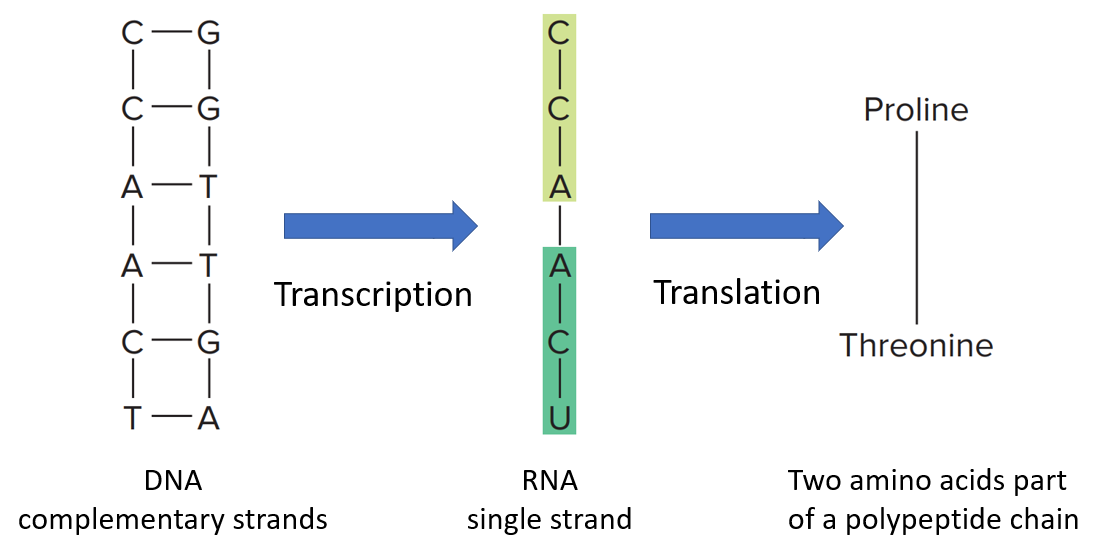
\includegraphics[width=.75\linewidth]{images/ch_2_protein_generation.PNG}
  \captionof{figure}{Conversion of DNA information into protein via the genetic code. Complementary bases in a DNA strand are split into a single RNA strand, which is read in pairs of three bases at a time (codon) to create a single amino acid in a polypeptide chain. Partially adapted from \cite{hartwell2008genetics}.}
  \label{fig:ch_2_protein_generation}
\end{figure}


Genes are long segments of DNA that encode information for a specific protein, which are the basic building blocks of all organisms. Proteins are made up of long chains of amino acids where the structure and function of the proteins are determinant on the order of these amino acids. Fundamentally proteins are manufactured using the information encoded in a gene through the process of transcription and translation, and collectively, this process is called gene expression. During transcription, the DNA present in a gene acts as a template to form an mRNA, which is a single-stranded structure consisting of one of every complementary base pair in the DNA. This is followed by translation where mRNA is used as a template to assemble a chain of amino acids such that each group of three bases in the mRNA called a codon creates one particular amino acid, as shown in Figure \ref{fig:ch_2_protein_generation}. Thus the order of bases in the DNA encodes for the order of amino acids in the protein and, in turn, its structure and function\cite{clancy2008translation}.

DNA is transferred from one generation to the other in all livings organisms through the process of self-replication where the double-helical structure of the DNA comes apart, and each of the complementary strands acts as a template in the production of its counterpart forming new pairs of DNA strands\cite{pray2008semi}. Although cellular error-checking mechanisms ensure that these new DNA strands are nearly identical to the original strand, mutations can occasionally occur. This can happen when a base at one position is replaced by one of the other bases or is entirely lost. Alternatively, insertions or duplications of more extended sets of base pairs can also happen. Other kinds of larger mutations such as chromosomal rearrangements can occur, including inversions, where a large segment of a chromosome is reversed in orientation or translocation where parts of chromosomes swap places between themselves\cite{hartwell2008genetics}. While most mutations that occur during duplication do not have an affect on a gene, they can however, in some cases, alter the function of the gene. This can be detrimental in some cases, leading to diseases such as cancer. While in some other cases such mutations can be beneficial by offering resistance to diseases or other environmental factors. 

\subsection{Comparative Genomics}\label{comparegenomics}

As these mutations accumulate over time, they lead to the divergence of species. Understanding how these changes could have occurred is a significant field of research in comparative genomics and has large scale implications such as improving the quality of human life\cite{collins2003vision}. Comparative genomics, as the name suggests involves comparing genome sequences of different species to identify regions of similarity and differences to gain information on the relatedness between the species genomically and functionally. The fundamental principle in comparative genomics remains simple in that sequences that encode for proteins and gene expression should be conserved in related species, whereas sequences that are responsible for differences between species will themselves be divergent\cite{hardison2003comparative}.

Comparative genomics can assist biologists in linking the phenotypic and genotypic properties of an organism to understand its different characteristics. For example, researchers combined the gene expression data of several plant sequences which have high gene duplication rates with evolutionary conservation data to improve on gene discovery \cite{hanada2008importance}. Also, the comparative analysis of genes and their regulatory pathways in the context of phylogeny provides scientists with a better understanding of how evolution happens at a molecular level\cite{soltis2003role}. However, the questions that are addressed by comparing genomes at different phylogenetic distances can vary \cite{hardison2003comparative}. For example genomic comparison between species that are separated by very long phylogenetic differences such as yeast(\textit{Saccharomyces cerevisiae}), worms(\textit{Caenorhabditis
elegans}), and flies (\textit{Drosophila melanogaster}) reveals that their genomes encode for many of the same proteins while the order of the genes and sequences are not conserved\cite{rubin2000comparative}. Whereas, comparison between more closely related species like Humans(\textit{Homo sapiens}) and Chimpanzees(\textit{Pan troglodytes}) reveal that the overall divergence between the two genomes is only 4\% and results are more oriented towards identifying the differences than the similarities \cite{varki2005comparing}. 

Comparative genomic studies are primarily focused around the study of homologous sequences, which are gene sequences that have shared ancestry where the extent of homology is determined by sequence similarity and are commonly referred to as homologs. Such similarity between DNA sequences can occur either because of a speciation event (a species diverges into two separate species) leading to orthologs or due to a gene duplication event (a gene is duplicated within the same genome) leading to paralogs \cite{jensen2001orthologs}. Research into such similar genes, especially in eukaryotic organisms can shed light on gene duplication events that lead to the creation of gene families\cite{rubin2000comparative}. Gene families are defnied large groups of gene sequences that are similar to each other while also having a similar function or gene expression. Usually, when a gene duplication occurs the new gene either remains inactive as a pseudogene or exists as a duplicate copy of the original gene performing the same function. Increased number of gene duplicates through natural selection can often lead to an increase in the protein synthesized by the gene. An example of this is the variation in gene copy number in the human salivary amylase gene (AMY1) responsible for starch hydrolysis in certain human populations\cite{perry2007diet}. A third scenario of gene duplication that can occur rarely is when the duplicated gene through mutations acquires a new function. An example of this is trocarin D gene of the Australian rough-scaled snake that acts as a toxin by coagulating the blood of its prey. Comparative genomic analysis of the trocarin D gene revealed that it is nearly identical to the coagulation factor(F) X gene present in the plasma of the snake responsible for blood coagulation to prevent bleeding when the snake is injured indicating that that the gene was recruited for a new function after a gene duplication event\cite{reza2007structure}.

\subsection{Synteny}
One of the ways in which homology can be inferred for understanding large scale duplication events is through studying collinearity of several genes, where both the gene content and order are conserved\cite{proost2011adhore}. Such long regions containing several genes that display collinearity in the order of Kilobases(Kb) to Megabases(Mb) are referred to as Synteny Blocks\cite{zeng2008orthocluster}. The word Synteny has greek origins with \textit{syn} meaning together and \textit{taenia} meaning ribbon and is used to indicate the presence of genetic loci on the same chromosome\cite{renwick1971mapping}. However, synteny can also occur between different chromosomes and nowadays is more commonly used to refer to ``gene loci in different organisms located on a chromosomal region of common evolutionary ancestry''\cite{passarge1999incorrect}.

With the availability of fully sequenced genomes of several model species, synteny analysis can reveal evolutionary adaptions and also improve the transfer of knowledge to non-model organisms that haven't been fully mapped\cite{zhao2019network}. Synteny analysis, particularly in angiosperms (flowering plants), can help in understanding the consequences of whole genome duplication in plant evolution\cite{adams2005polyploidy} as shown in the analysis of polyploidy in Thale cress(\textit{Arabidopsis thaliana})\cite{seoighe2003turning}. This state of polyploidy where an organism contains more than two sets of homologs is a widespread occurrence in plants  due to several whole-genome duplication events at diverse temporal scales but is rare in mammals with evidence of the last whole genome duplication event occurring almost 500 million years ago\cite{adams2005polyploidy,panopoulou2005timing}. However gene collinearity is conserved to a greater order in mammals than plants thus making synteny analysis at smaller scales called microsynteny much more feasible\cite{zhao2019network}. In this way, synteny analysis can be adapted to a wide range of scenarios and evolutionary scales based on the underlying question.

\subsection{Analysis Pipeline}

Synteny analysis consists of three major steps: Sequence Alignment, Synteny Detection, and Data Visualization. Although SynVisio focuses on the last step, we will take a brief look at the other preceding steps. Before analyzing synteny between two or more organisms their genomes need to be sequenced and assembled at least partially into scaffolds. This process is then followed by similarity detection between the two genomes through sequence alignment.



\subsubsection{Sequence Alignment}
Sequence alignment is extensively used in computational biology to assess the similarity between DNA, RNA, and protein sequences. Fundamentally sequence alignment works by arriving at an optimal alignment through a scoring mechanism, where gaps are introduced in one of both of the sequences but penalized accordingly, as shown in Figure \ref{fig:ch_2_sequence_alignment_multi}. A gap at any position in the final alignment is an indication of an insertion or a deletion and is penalized because these events are far less likely to occur than mutations. The validity of sequence alignment results is dependant on the alphabet size of the sequences  as protein sequences can contain up to 20 different amino acids, whereas DNA sequences only contain four different bases leading to better alignments in proteins. There are two major types of sequence alignments, and they are used in different scenarios. The first type of sequence alignment where an optimal match is found by aligning the two entire sequences end to end is called Global sequence alignment and is used to compare homologous sequences. The second type of alignment that looks at smaller sections or sub-sequences to find a match is called Local sequence alignment and is used in looking for patterns in a sequence when comparing it with a larger set of sequences such as those in a database. 

\begin{figure}
  \centering
  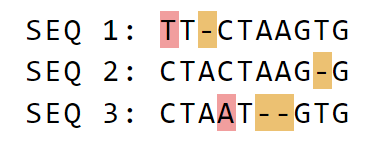
\includegraphics[width=.45\linewidth]{images/ch_2_sequence_alignment_multi.PNG}
  \captionof{figure}{Sequence alignment of sequences `TTCTAAGTG',`CTACTAAGG' and `CTAATGTG' with mismatches and gaps highlighted in red and orange respectively.}
  \label{fig:ch_2_sequence_alignment_multi}
\end{figure}


Every sequence alignment is centred around an optimization problem and early alignment techniques such as the Needleman and Wunsch Method \cite{needleman1970general} used a dynamic programming approach to arrive at the optimal alignment. Dynamic programming is a computational strategy that recursively breaks larger problems into smaller sub problems and reuses the results of previously solved sub problems to arrive at a solution of the larger problem. A variation of the Needleman and Wunsch Method for local sequence alignment is the Smith-Waterman algorithm\cite{smith1981identification} that uses a matrix based scoring scheme for comparing sub sequences.
However, the time complexity of such methods increases exponentially when searching for sequences in large databases leading to the adoption of heuristic methods to align sequences such as the FASTA (Fast-All) algorithm \cite{lipman1985rapid}. Although this algorithm is no longer in use, the name FASTA is still used for a popular file format in bioinformatics, for representing nucleotide and protein sequences as a series of single-letter characters.

BLAST (Basic Local Alignment Search Tool) is a popular local sequence alignment tool that acts as a direct successor to the FASTA algorithm being more time-efficient and operating on the same file format\cite{pertsemlidis2001having}. It operates by identifying small query words that contain three nucleotides or amino acids for protein sequences in a particular order based on their occurrence along the sequence and closeness to other similar words. It then expands on these words on either direction based on searches from target databases rated by scoring matrix. Blast by default uses BLOSUM62 (Block Substitution Matrix) as its scoring matrix which ensures that even more distantly related sequences are detected but other matrices such as PAM250 (Point Accepted Mutation) can also be specified.



\subsubsection{Synteny Detection Tools}

The next step after detecting the similarity between two sequences is the actual synteny detection, as alignment results are only pairwise between sequences and need to be grouped into larger blocks to look for patterns. Although Synteny detection tools differ in their operating file formats and computational efficiency, they broadly work by combining positional information of genes along a genome sequence with pairwise BLAST results to construct chains of collinear gene pairs. Grouping neighboring gene pairs that match is one way of detecting syteny\cite{wang2012mcscanx} that is implemented in tools such as OrthoCluster\cite{zeng2008orthocluster},TEAM\cite{luc2003gene} and ADHoRe\cite{proost2011adhore}. These tools are, however, outdated and are not efficient in detecting syntenic blocks with conserved gene order, especially in scenarios that might include chromosomal rearrangements and tandem duplications\cite{wang2012mcscanx}. A new class of synteny tools such as MCScanX\cite{wang2012mcscanx}, DAGChainer\cite{haas2004dagchainer}, and CYNTENATOR\cite{rodelsperger2010cyntenator}, that utilize a dynamic programming approach to create chains of pairwise collinear genes around anchor genes are much more efficient at detecting collinear syntenic blocks. Some such as MCScanX even offer downstream analysis tools with visualization results, as shown in Figure \ref{fig:ch_2_synteny_plots}.     

\begin{figure}
  \centering
  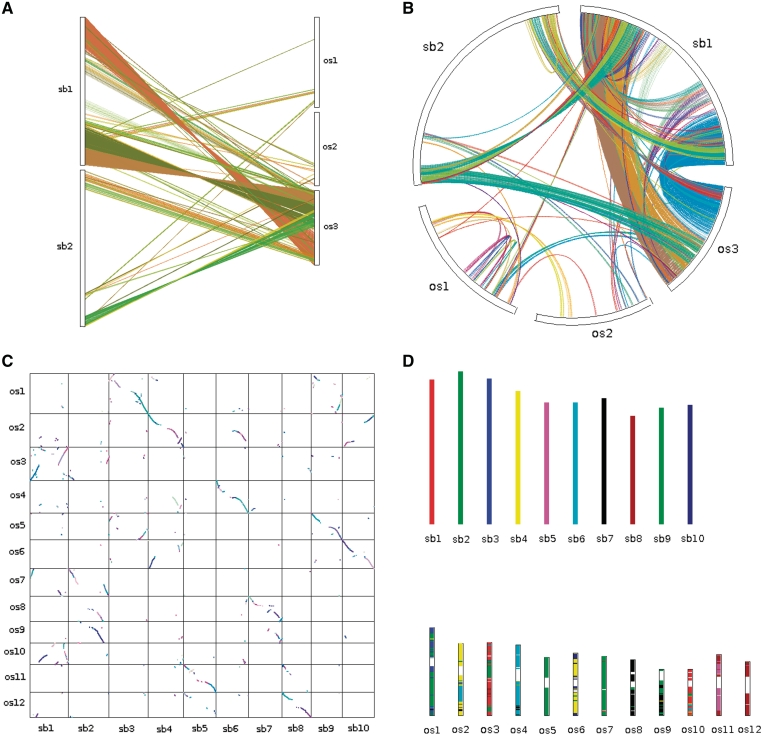
\includegraphics[width=.75\linewidth]{images/ch_2_synteny_plots.jpg}
  \captionof{figure}{Different types of plots visualizing synteny generated by MCScanX : (A) dual synteny plot, (B) circle plot, (C) dot plot and (D) bar plot, From Wang et al.\cite{wang2012mcscanx}.}
  \label{fig:ch_2_synteny_plots}
\end{figure}

\section{Genomic Visualizations} 
With the advent of rapid genome sequencing systems, genomic data is being generated at an exponential pace that is not being met in terms of innovations in data analysis systems that can help researchers in understanding these ever increasing data streams. Visualization systems however can play a critical role in bridging this gap in data exploration as humans are intuitively good at finding patterns. As research in this field becomes increasingly data-driven, visualization systems can aid researchers, particularly in generating a hypothesis and iteratively refining it by encoding genomic information through visual cues in the form of shapes and colours\cite{nusrat2019tasks}. Genomic visualization systems can be used in several scenarios, such as analyzing sequence data at different resolutions and browsing annotations and reference tracks or in comparing sequences from different organisms\cite{nielsen2010visualizing}. However a major challenge in this field remains in determining the right graphical representation based on the genomic context and data under exploration. In this section, we first explore the different kinds of visualizations systems and techniques that are used in representing genomic data at the sequence and genome level. We then look particularly at systems that are used in exploring sequence similarity at different resolutions and finally give a brief overview of the current synteny visualization systems that are available and their merits and demerits.

\subsection{Sequence and Genome Browsers}
Visualizing genomes at the sequence level is primarily done by representing sequences
as a series of letters organized on a linear scale from left to right in the reading order. Additionally, sequences that are longer are stacked vertically. This ordering of bases or amino acids is meant to aid researchers in identifying discrepancies by quickly scanning down the sequence along its length, especially in scenarios involving comparing read alignments. Visual cues such as emphasis through colors are further used to highlight erroneous bases in some sequence analysis tools\cite{consed,ewing1998base}. Other tools like IGV (Integrative Genomics Viewer)\cite{thorvaldsdottir2013integrative} and Hawkeye\cite{schatz2007hawkeye} opt for a simpler representation by only visualizing discrepancies. Sequence visualization systems are also used to interpret and refine the results of sequencing systems where visual cues are provided to highlight gaps, mismatches, and the order of repeats\cite{bonfield1995new,consed}. In some systems such as Consed\cite{consed}, information is visualized in pairs that are color-coded so that structural variations such as insertions, deletions and inversions are also considered, and additional information is provided in the form of annotations of amino acids translations to identify miss-assemblies. Finally, some tools like the ABySS-Explorer provide an assembly graph overview for high-level inspection of the assembly instead of focusing on the local sequence mismatches\cite{nielsen2009abyss}. 


\begin{figure}
  \centering
  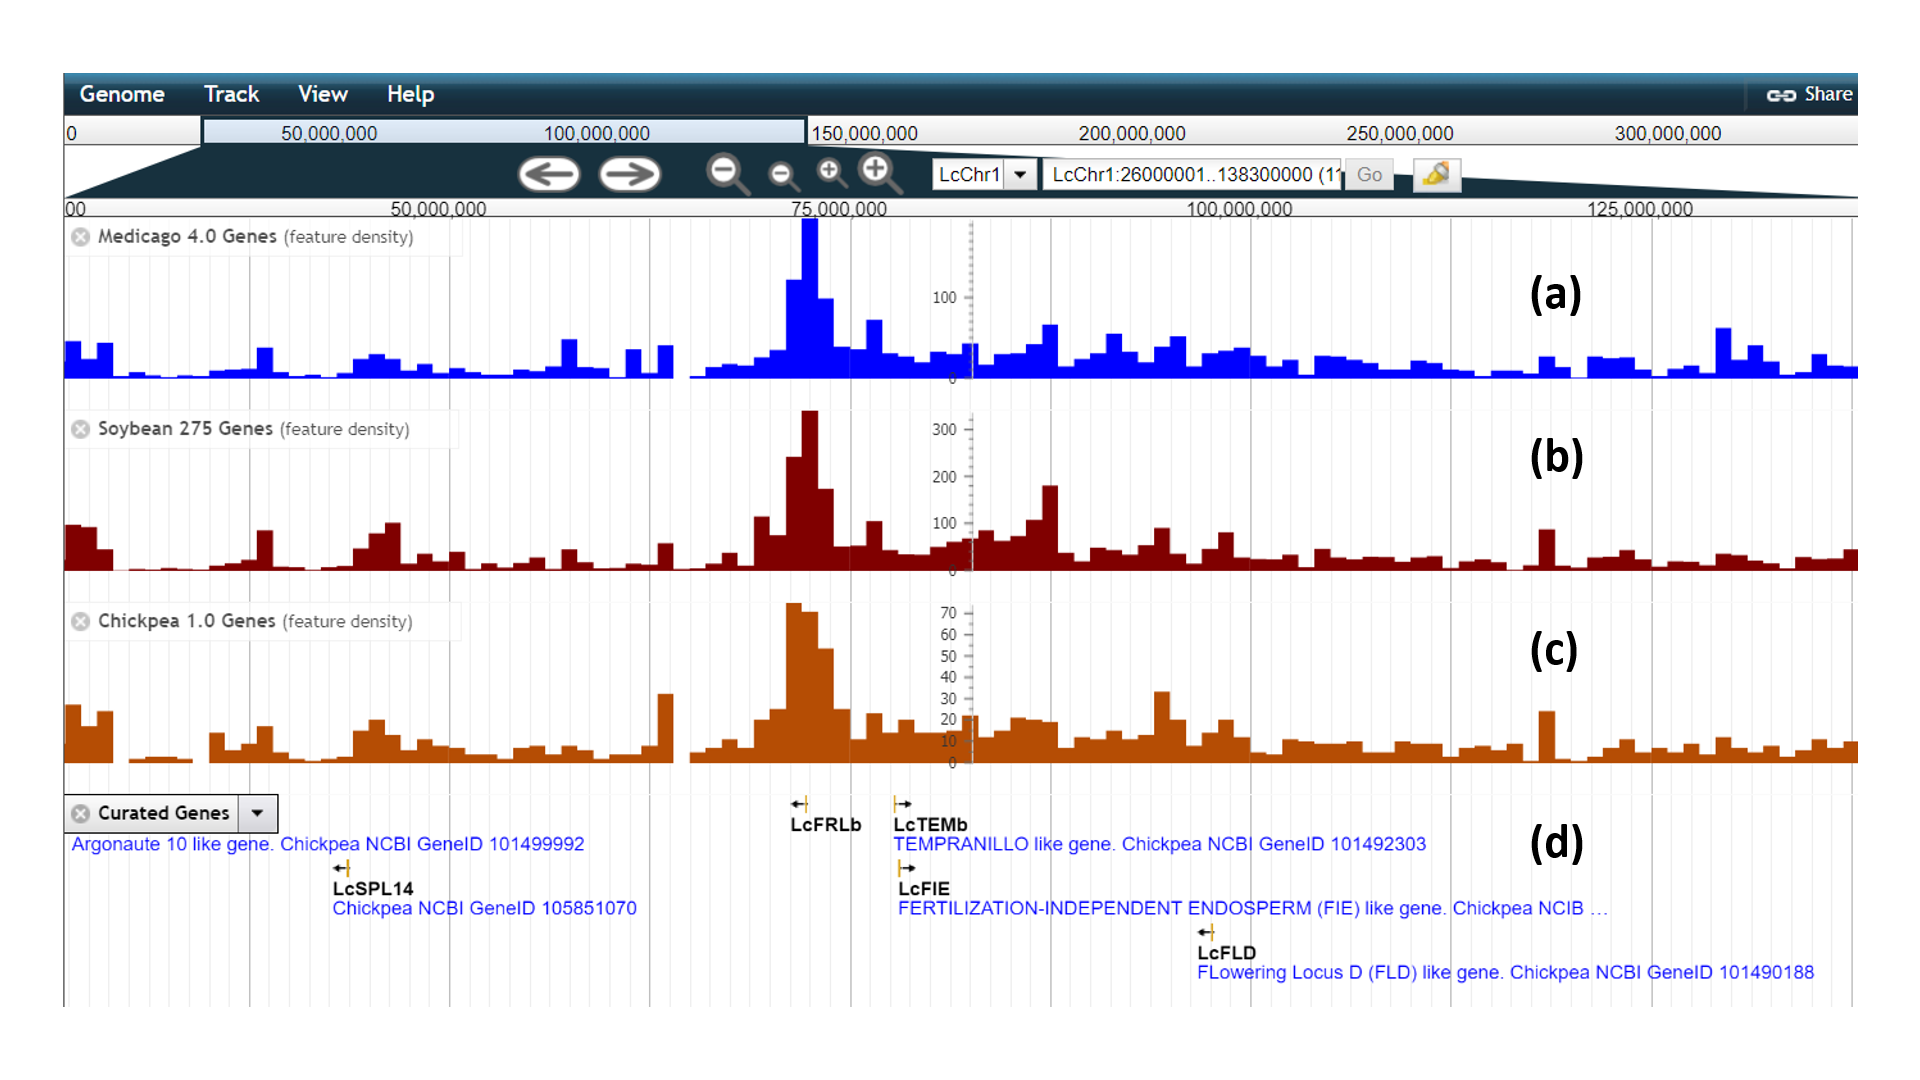
\includegraphics[width=1\linewidth]{images/ch_2_jbrowse.PNG}
  \captionof{figure}{JBrowse used to compare gene densities between (a) Barrel Medic(\textit{Medicago truncatula}), (b) Soybean(\textit{Glycine max}) and (c) Chickpea(\textit{Cicer arietinum}) in relation to curated genes encoding for prominent phenotypes (d) generated through KnowPulse \cite{sanderson2019knowpulse}. }
  \label{fig:ch_2_jbrowse}
\end{figure}


Once the short sequence reads are assembled into a single large genome, a different set of visualization tools are required that are focused around identifying particular regions of interest. A genome sequence in its entirety can acts a reference against which several features such as gene densities, SNPs, and repeats can be mapped. This form of analysis is increasingly being used in a wide range of browsers that were developed to disseminate information and provide a platform for the exploration of several genomes that are sequenced for model organisms such as GBrowse\cite{stein2002generic}, Ensembl Genome Browser\cite{stalker2004ensembl} and UCSC Genome Browser\cite{ucscgenome}. These browsers work by displaying a requested portion of the genome with several annotation tracks stacked vertically against each other along a reference axis. The annotation tracks can contain different kinds of information such as positions of single nucleotide polymorphisms, regions with regulatory elements, location of important genes, as shown in (d) of Figure \ref{fig:ch_2_jbrowse} and can be toggled on or off depending on their requirement in the analysis. The information is visualized at several resolutions from hundreds of base pairs all the way upto tens of thousands with the ability to move along the genome horizontally and zoom in and out of a particular region. Some genome browsers even offer the ability to search for a particular gene by looking up its position in the underlying database\cite{nielsen2010visualizing}. 

Finally, additional visual representations such as summary views (of copy number variations) in the context of biological pathways are also provided in certain browsers like UCSC Cancer genomics browser\cite{ucscgenome}, allowing researches to associate clinical features with genomic data directly. This form of a genome overview that preserves global context while still allowing researchers to explore smaller chromosome level entities is also present in Gremlin, a tool that offers a novel visual model for exploring structural variants and rearrangements\cite{o2010gremlin}.  

With an increase in the volume of data being generated, genome browsers are being adopted towards a decentralized model where processing power is distributed between the server and the client's browser. Information is retrieved only when needed for the resolution and the region that the user is interested in and visualizations are generated on the fly in the client-side. This reduces the load on the server substantially and modifies it to serve purely as a database to lookup information when necessary. This form of rendering in the client can offer a smoothly animated experience while navigating a genome through panning or zooming. It also ensures that there are no disruptions to a user's sense of location by averting incongruous transitions that occur when large data sets are being loaded and traversed. An example of such as browser is JBrowse that offers superior visualizations as shown in Figure \ref{fig:ch_2_jbrowse} along with significantly less server overhead compared to other genome browsers\cite{skinner2009jbrowse}.
Certain genome browsers take this decentralized model a step further by offering connectivity to data stored locally on a user's computer\cite{ucscgenome,saito2009utgb}. This can provide a personalized experience when dealing with sensitive data in situations where storing data on a remote server may not be viable. 

\subsection{Comparative Genome Browsers}
With the ability to sequence multiple genomes within a short span of time, a new field of research has emerged that centers around comparing genomes instead of looking at them in isolation and is called comparative genomics, as discussed earlier in \ref{comparegenomics}. Regardless of the data type or domain, comparison is a common task in data analysis and visualization, when there is a need to understand the relationship between a given set of items.\cite{gleicher2017considerations}. Visual comparison ,in particular, has been shown to improve the understanding of data in several charts and designs explored by Tufte\cite{tufte1990envisioning} along with specific examples centred around Playfair's use of line graphs to demonstrate the change in stock prices in relation to wars\cite{costigan1990william}. In the field of genomics, comparison can aid biologists in a diverse set of tasks such as identifying functional elements, studying large scale rearrangements and genome evolution, and finally refining results of genome assembly systems through reference genomes\cite{nielsen2010visualizing}. Several systems have been built to address each of these tasks through visual comparison at different genomic scales as sequences can be compared at the nucleotide level all the way up to the whole genome level.

At the nucleotide level, researchers compare sequences to identify the location of mutations, insertions and deletions, and most visualization tools designed for such analysis achieve this by representing alignments on a linear scale. Visual cues are provided by colouring each of the four nucleotides in a categorical colour scale, and the sequences are presented in a linear layout, usually in a stacked arrangement. Some of these tools like JalView(JV2)\cite{waterhouse2009jalview}, are enhanced with interactive features that let users sort, filter, highlight, and edit multiple sequences in real time. Jalview also lets users overlay sequence features onto the alignment and render extra positional features through transparent or opaque shading over specific regions of an alignment. AliView is a similar tool that works for extremely large datasets through an indexing process and offers support for multiple file formats\cite{larsson2014aliview}. However, JalView and AliView are limited in usability being desktop applications but recent tools such as MSAViewer\cite{yachdav2016msaviewer} and JSAV(JavaScript Sequence Alignment Viewer)\cite{martin2014viewing} have been designed to work across the internet as web applications with the same set of features.

When comparing sequences at higher levels, researchers look for large scale rearrangements. Due to the higher resolution of data, genomic features are grouped into contiguous blocks on each chromosome called syntenic blocks where conservation is implied through the similarity and relatedness between these blocks.
Several strategies have been explored to graphically represent syntenic blocks both at the chromosome and the whole genome level. The earliest examples for representing synteny involve the adaptation of dot plots used for comparing local alignments for larger sequences. Most of these tools primarily perform the actual genome level comparison and present their results through dot plots for closer inspection such as DAGChainer\cite{haas2004dagchainer} and VISTA plots of the MUMmer alignment tool\cite{kurtz2004versatile}. Dot plots are two dimensional representations, where genomes of two organisms are presented along the \textit{x} and \textit{y} axes respectively. Gridlines are used to show the chromosomal boundaries, and every similar gene is represented as a point and large collinear blocks of genes are shown through lines. Such matrix-based representations are extremely good at identifying genome rearrangements, as duplications show up as secondary lines parallel to the diagonal and reversals end up being straight lines that are perpendicular or inclined away from the diagonal. While these plots offer great genome level summaries of alignments, they cannot be extended for multi-way comparisons between several genomes or used to identify smaller rearrangements at the chromosome level easily.

\begin{figure}
  \centering
  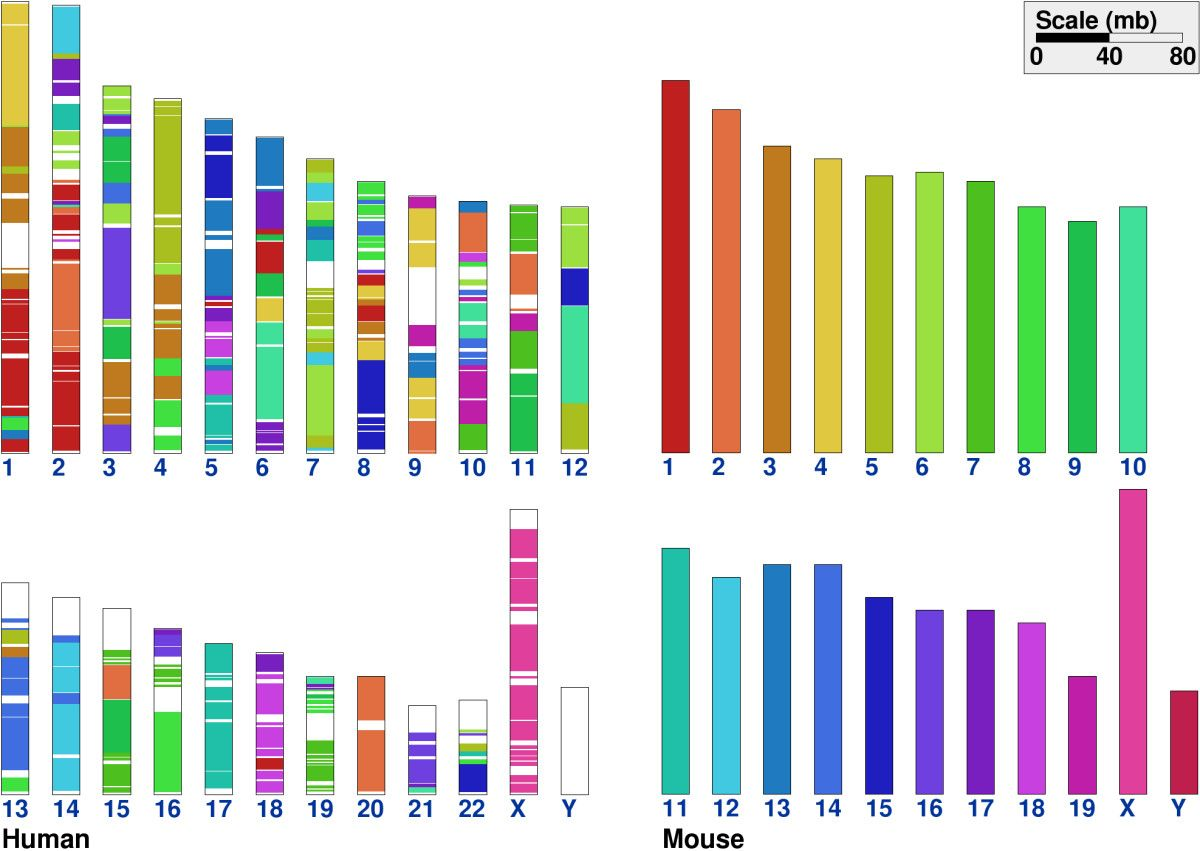
\includegraphics[width=0.75\linewidth]{images/ch_2_cinteny_pill.jpg}
  \captionof{figure}{Visualization of synteny between human and mouse genomes shown by a pill based design in Cinteny. Image extracted from \cite{sinha2007cinteny}. }
  \label{fig:ch_2_cinteny_pill}
\end{figure}

Another representation of synteny that has been used extensively in tools such as Cinteny\cite{sinha2007cinteny}, Sybil\cite{crabtree2007sybil} and MEDEA\cite{nusrat2019tasks} is the pill-shaped ideogram design of chromosomes. In this design, chromosomes of the source genome are represented as pill shaped rectangular blocks that are color coded on a categorical scale and chromosomes in the target block are represented as similar pills with varying sizes based on their genomic sizes. Syntenic regions in the target are then represented through color coded bands where the color is determined by the source chromosome the alignment belongs to, as shown in Figure \ref{fig:ch_2_cinteny_pill}.
The choice of representing a chromosome as a rectangular pill is based on a karyogram representation of chromosomes in biological literature, but information about the position of the centromere is omitted, and the ``X" or ``V" shaped design is adopted into a single cylinder shaped like a small pill. While the use of colours makes it easier to quickly identify similar regions and their distribution in the target genome, in comparison to a dot plot, this representation loses some information such as the orientation of the aligned blocks and their relative position in the source genome. Tools like Apollo partially solve this problem by extending this representation by also linking the colored segments in the reference genome with its corresponding loci in source chromosome through lines and interleaving the source and target regions \cite{lee2009apollo}. Mauve follows a similar approach but uses a linear layout and stacks the sequences parallel to each other, using connections to encode conservation\cite{darling2004mauve}. A significant problem with this representation, along with other designs that rely extensively on color is that it cannot be extended for a large number of chromosomes as humans cannot intuitively distinguish beyond ten colours \cite{tufte1990envisioning}. Further the choice of colors is extremely important as colors need to be visually distinct unlike the colors chosen in tools like Cinteny\cite{sinha2007cinteny} as shown in Figure 2.5. The colors used in chromosomes 6-9 and 12-15 are very close to each other in the green and blue spectrum, respectively, that its hard to distinguish them when the colored bands in the target are small and close to each other. 

A third form of representation that has recently gained a lot of traction due to its aesthetically appealing visuals is the Circos style plot\cite{krzywinski2009circos}. In these plots, genomes are represented as arcs presented in a circular layout. Syntenic regions are shown as lines connected through the middle of the circle. Additional tracks representing other information such as copy number variants and SNPs are presented through outer circles along the genome. The circular arrangement is meant to reduce visual clutter that can arise in a linear stacked arrangement when multiple linked regions represented through lines cross each other, causing a web of lines that are hard to distinguish and follow. Tools like Circa that generate these plots can be configured to use a diverse set of color schemes and visual representations like histograms, heat maps, line charts, and scatter plots for the outer tracks\cite{circa}. 

\begin{figure}
  \centering
  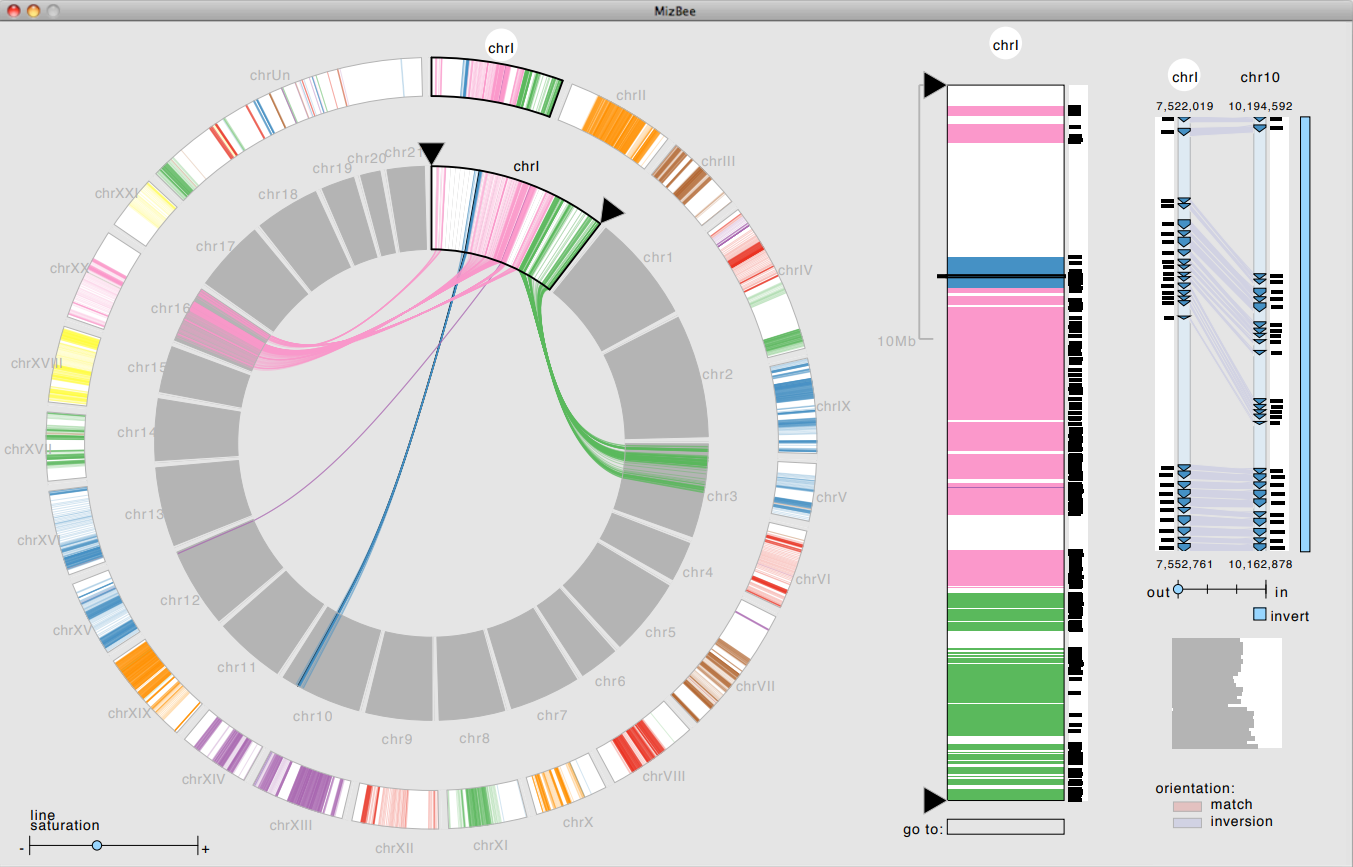
\includegraphics[width=0.75\linewidth]{images/ch_2_mizbee.PNG}
  \captionof{figure}{Synteny visualization as shown by Mizbee. Image extracted from \cite{Meyer2009}. }
  \label{fig:ch_2_mizbee}
\end{figure}

Mizbee is an example of a standalone synteny browser that combines the circular layout with a linear arrangement to present syntenic information at different scales. Mizbee presents genomic conservation through a combination of connections and color encoding in three linked views that are presented next to each other, as shown in Figure \ref{fig:ch_2_mizbee}. In the genome view, chromosomes are presented as arcs in two concentric rings. The source chromosomes are presented in the outer ring, and the inner ring contains the target chromosomes arranged around a copy of the selected source chromosome. Conservation is then encoded through links connecting the collinear blocks inside the inner ring with additional encoding in the form of colour. The circular layout reduces visual clutter, which is further addressed through edge bundling of contiguous blocks that go to the same destination chromosome. Noisy data in the inner ring can be explored by selecting a particular region which is then presented in a chromosome view that is present in the middle of the display as seen in Figure \ref{fig:ch_2_mizbee}. The color coding at this level is similar to the genome view but connections are presented in a vertical layout that supports precise spatial analysis. The final view called the block view presents the individual genes in a particular collinear block through connected ribbons along with their orientation encoded as directed triangular blocks. Mizbee is the first of many such browsers that have been developed to go beyond simple chart generation and act as a complex analysis tool that can present conservation through a combination of multiple visual representations. Mizbee, however, doesn't perform the actual synteny detection and relies on a formatted input dataset. This requires researchers to first detect synteny through a detection tool like DAGChainer, MCScanX or iADHoRe and then modify the output to match the input format of Mizbee. Mizbee also doesn't offer support to supplement the generated visualizations with tracks for additional information that provide biological context and is limited in its usability being a standalone desktop tool. 

mGSV (Multi Genome Synteny Viewer) is a synteny viewer that works similar to Mizbee by visualizing synteny through a combination of visual representations but is available as a web based tool\cite{revanna2011gsv}. It lets users upload pre-computed syntenic data in a tab-delimited format and also accepts an extra annotation file to show additional genomic features as an annotation track. The system, however, works in a distributed model where syntenic information is stored in a remote database and charts are generated in the server and fetched based on user interactions in the browser. This server based model can cause data security issues and also add unnecessary network delay into the analysis, making it a time consuming process. SimpleSynteny is another such web based tool that represents information in a horizontal linear layout using a combination of colored bars and connected ribbons for representing genomic conservation\cite{veltri2016simplesynteny}. It however accepts FASTA files as input for the genomes and uses BLAST\cite{blasttool} on a remote server to align the sequences into collinear blocks. While this does improve the usability of the tool, synteny detection is a resource intensive process that can place a load on the server, especially for large genomes, and is best done on desktop machines that are computationally powerful.

A recent set of synteny browsers that are web based and also let users download visualizations as image files are Synteny Portal, MultiSyn, and AccuSyn. Synteny Portal uses alignments that are pre-built and stored in the UCSC genome browser database but cannot be extended for custom sequences\cite{lee2016syntenyportal}. MultiSyn\cite{baek2016multisyn} is similar to SimpleSynteny but relies on only protein sequences as its input and detects synteny on the server using MCScanX\cite{wang2012mcscanx} a popular synteny detection tool. AccuSyn\cite{accusyn} is the latest tool on the market that lets users upload synteny results of MCScanX and generates visualizations in real-time on the client-side. It presents conservation similar to Mizbee in two linked views with a circos style layout with connected ribbons for the genome level and a vertical layout with connected glyphs for the block level, as shown in Figure \ref{fig:ch_2_accusyn}. AccuSyn also lets users upload several annotation tracks with the ability to customize the color scale and the visual representation of the track.

\section{Interaction Techniques in Genomic Visualizations}
Visualization for data exploration and analysis primarily involves the graphical representation of the data, however, user interaction still plays a major role in both navigation and assessment of the generated visualizations.  In this section, we first explore the different techniques that are used in genomic visualization tools to manipulate both the underlying data and the graphical interfaces for data exploration. We follow this with a discussion of how data analysis can be improved with the support for revisitation and tracking user interactions.

\begin{figure}
  \centering
  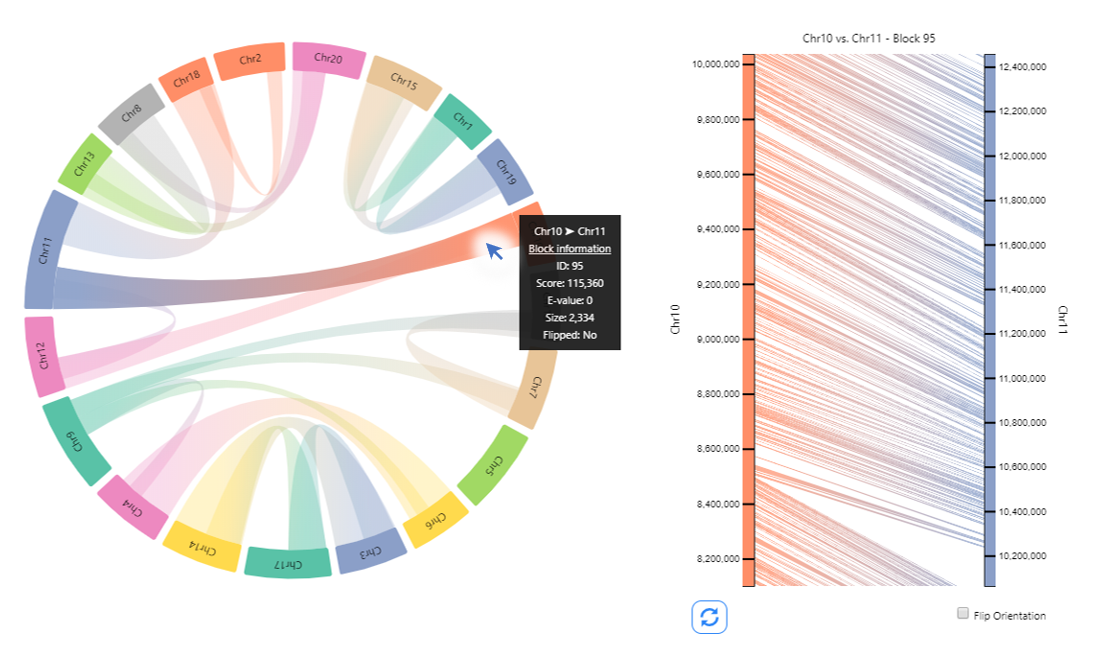
\includegraphics[width=0.95\linewidth]{images/ch_2_accusyn.PNG}
  \captionof{figure}{Multi View Synteny Exploration in AccuSyn\cite{accusyn} showing conservation in \textit{Camelina sativa} with a single collinear block highlighted between Chromosomes 10 and 11. }
  \label{fig:ch_2_accusyn}
\end{figure}


\subsection{Multi-Linked Views}

Although visual encoding of information through static visualizations can assist users in simple data analysis tasks, the usability of such a system falls short when its utilized for complex tasks and activities\cite{tominski2015interaction,dix1998starting,pike2009science,piringer2009multi,yi2007toward,sedig2013interaction}. The efficacy of such a system can be considerably improved by providing interaction mechanisms that can modify the graphical representations based on the different tasks, users, their expertise and other contextual factors\cite{sedig2013interaction}. Complex analysis tasks go beyond basic visual perception, that is needed for simple tasks, and often require extended cognitive processing from the user. Interaction mechanisms are important in these scenarios as such complex tasks can be achieved through engaging user actions that in turn enhance cognitive processing\cite{sedig2013interaction}. Research, in particular, has also shown that viewing the same underlying data in multiple representations can help users in forming an accurate mental model of the data\cite{larkin1987diagram,stenning1995cognitive,sedig2005designing,wang2000guidelines}.

In the context of comparative genomic visualizations, some of the earliest examples of enhancing basic charts with interaction techniques include support for zooming into a two dimensional dot plot for closer inspection of a particular region in Dagchainer\cite{haas2004dagchainer}. Tools like SynMap2\cite{haug2017synmap2} belonging to the CoGe(Comparitive Genomics)\cite{coge} Web Platform have also extended the features to explore such dot plots through mouse-based scrolling and panning similar to modern mapping platforms like google maps. This form of zooming into data for exploration is also used in several other tools and is part of the larger design principle proposed by Shneiderman\cite{Shneiderman96theeyes} called the visual information seeking mantra. The principle summarizes the essential elements of interaction with visualization systems as: overview first, zoom and filter, then details-on-demand. In synteny visualizations an overview can often mean presenting comparative relationships at the whole genome scale by grouping collinear blocks. At this level visual encoding is used for distinguishing the different chromosomes the collinear blocks belong to and their size, proximity and position. Mizbee is an example of a tool that follows all four essential steps of the visual information seeking mantra\cite{Meyer2009}. It presents overview level information in the circos style plot, as shown in Figure \ref{fig:ch_2_mizbee} and specific sections of the genome can be zoomed and filtered through markers placed on the overview plot. Additional details of individual gene blocks that make up larger collinear blocks are brought up on-demand through user interactions at the higher levels either in Genome View or the  Chromosome View. 

mGSV(Multi Genome Synteny Viewer) is another such tool that provides a summary view showing genomic conservation at the genome level in a circos style plot\cite{revanna2011gsv}. Unlike Mizbee, which lets users explore in through multi-linked views mGSV provides two operating modes, a pairwise view mode, and multiple view mode. In the pairwise mode conserved regions are shown between adjacent genomes and interactions are centered around selecting specific regions of the different genomes and reordering the genomes. In the multiple view mode, conserved regions connecting all visible genomes are shown and interactions are focused around toggling the visibility of genomic regions to ensure they do not overlap over other genomes in the stacked layout. mGSV also employs a heuristic algorithm to optimizes the layout of the genome order based on the size of the conserved regions to minimize visual clutter. However, this 
can often create layouts that while being visual clear may not provide the right biological context. AccuSyn solves this problem through a novel Human-in-the-loop methodology\cite{accusyn}. It uses a simulated annealing heuristic to arrive at the optimal layout and also takes into consideration the position of chromosomes set by the users through manual dragging and flipping operations. This can ensure that as users explore the syntenic relationship between the genomes, they can tune the algorithm to arrive at an uncluttered layout that also has meaningful insights.

\subsection{Interaction History and Revisitation Support}

Exploring genomic information at different resolutions can be problematic due to its volume, complexity, and limitations in the availability of visual space but can be addressed through effective interaction techniques. However, relying on interaction mechanisms to navigate visual spaces can come with its own set of problems, one of which is memorability. Memorability is the degree to which users can retain information about the position of objects and markers in a visualization and revisit them. Revisitation is important in data exploration as it can help users retrace their steps and is part of the \textit{history} stage of the information seeking mantra presented by Schneiderman\cite{Shneiderman96theeyes}. However, revisitation can be affected by interaction techniques that require users to switch between graphical representations or zoom into a particular region and cause them to lose context of their previous position. Humans primarily rely on spatial cognition to remember the locations in objects in information workspace tasks but context switching visual systems can disrupt this ability\cite{datamountain}. Similarly interactive techniques such as fisheye views that work by distorting the original visualizations can also impair spatial memory as shown by Skopik and Gutwin\cite{gutwin2003finding}. 


One of the method in which this problem can be addressed is by storing the interaction history of the system and presenting it as a graphical abstraction either in the visual system itself or as an external panel. Not only can interaction history show the historical actions performed by a user it can also provide information on the actions performed so far that have led to the current state of the visual system. This interaction history can be provided indirectly through a history widget panel or by direct encoding into the visualization through the notion of \textit{readwear} or \textit{visitwear}. An example of  direct interaction history encoding in a visualization system is the visitwear mechanism developed by Skopik and Gutwin for fish eye views to highlight visited nodes. \textit{HindSight} is a similar direct encoding design framework that proved that users were able to visit more data points and recall novel insights by using their framework\cite{feng2016hindsight}. It encoded interaction history by making visited charts in a multi plot system appear darker or relied on existing visual encoding in line-charts and made visited lines slightly larger.

The second indirect encoding method for interaction history stems from research in visual analytics for supporting \textit{provenance} - which is the history of steps that led to a particular result in a data analysis workflow\cite{gotz2009characterizing,freire2008provenance}. The concept of provenance of visual history is centered around systems like the \textit{VisTrails} tool\cite{bavoil2005vistrails} that let users save visual outputs and revisit earlier states in the data analysis process. The notion of the earlier states termed as \textit{graphical histories} is explored further by Heer et al.\cite{heer2008graphical} in their graphical history interface for the Tableau visualization system.
In the context of genomic visualizations to the best of our knowledge direct encoding of interaction  history has not been explored but some recent synteny visualization tools like AccuSyn have offered partial support for revisitation through indirect encoding by letting users manually snapshot states of the system and revisit them through a history panel.